\def\E{4}
\def\ttau{0.015}
\def\RR{1333.3}
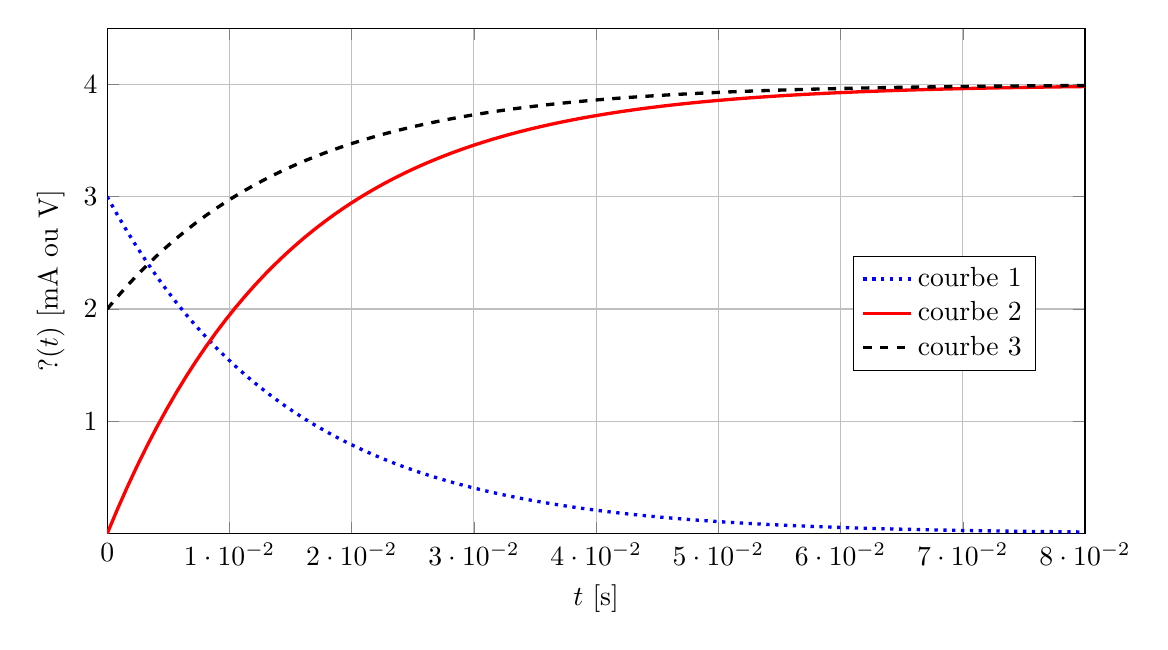
\begin{tikzpicture}
          \begin{axis}[xmin=-0,xmax=0.08,ymin=0,ymax=4.5, width=14cm,height=8cm, grid=both,ytick={1,2,3,4} ,xlabel={$t~[$s$]$},ylabel={$?(t) ~[$mA ou V$]$},
        ylabel near ticks,
        xlabel near ticks,
        scaled x ticks=false,
      legend style={at={(0.95,0.55)}}
]
              \addplot[very thick,blue,,dotted,domain=0:0.08,samples=100] {1000*\E / \RR*(exp(-x / \ttau ))}; % *1000 pour avoir des mA
              \addplot[very thick,red,domain=0:0.08,samples=100] {\E*(1.0 - exp(-x / \ttau) ) };
              \addplot[very thick,black,dashed,domain=0:0.08,samples=100] {\E*(1-0.5*exp(-x / \ttau))};
              \legend{courbe $1$,courbe $2$, courbe $3$}
          \end{axis}
\end{tikzpicture}